\newpage
\section{Problema 2: Algoritmo Exacto para List Coloring}

\subsection{Descripción de la problemática}
En esta oportunidad se nos pide resolver el problema List Coloring que consiste en (si es posible) colorear un grafo de forma que ningún nodo tenga el mismo color que un nodo adyacente, respetando la lista de colores de cada nodo, lo cual quiere decir que no se le puede asignar un color a un nodo si este no pertenecía a su lista de colores posibles. 

\subsection{Resolución propuesta y justificación}

Para desarrollar un algoritmo exacto para este problema decidimos usar backtracking y de esta forma recorrer todas las opciones de colores y poder encontrar la solución si esta existe.\\

Como el enunciado pide que al llegar a un caso de 2-List Coloring se utilice el algoritmo del primer punto, decidimos cambiar el enfoque de la resolución para poder adaptarlo a instancias del ejercicio 1. Por lo tanto en lugar de usar el enfoque convencional que sería fijar un color para cada nodo y ver si es solución, optamos por recorrer todos los nodos del grafo fijando dos colores por cada uno y al llegar al último nodo llamar a 2-list Coloring para que chequee si con esa configuración de colores hay solución. Si la respuesta es $"X"$ entonces se selecciona el siguiente color del último nodo y se vuelve a probar. Cuando se acaban los colores del último, se elije el próximo color del ante último y se vuelve a empezar de cero con los colores del siguiente y así hasta que se prueben todos los colores de todos los nodos. De esta forma siempre se llega a un caso base que es resoluble por 2-List Coloring.\\

Para evitar repetir colores se utilizan dos iteradores, el primero (\emph{it}) siempre arranca desde el primer color de la lista y el segundo (\emph{it2}) arranca desde el índice siguiente al de \emph{it}. De esta forma se generan todas las permutaciones de dos colores sin repeticiones ni omisiones.


\subsubsection{Podas}

\begin{itemize}
	\item La primer poda que se realiza es la de ordenar la lista de nodos de forma que queden primero los nodos con menor cantidad de colores ya que de esta forma si se eligen los colores de un nodo $a$ con dos colores primero y luego se pasa a uno $b$ de cinco, se estaría recorriendo el subgrafo que no contiene a $a$ dos veces en lugar de las cinco que se recorrería si estuviera primero el nodo $b$.
	\item Una poda también sería no llamar a 2-List Coloring con un nodo que tenga los colores $\{0, 1\}$ y luego volverlo a llamar con el mismo nodo con los colores $\{1, 0\}$ por ese motivo se recorren las listas de colores de la forma que explicamos antes.
	\item En el caso que el nodo original tenga un solo color, se llama directamente a 2-List Coloring, evitando entrar al while.
	\item Si se llega a una solución, se corta el backtracking y se devuelve esa. De esta forma en el caso promedio y mejor, no se recorrería todo el árbol de soluciones ya que no necesita encontrar todas las posibles.
\end{itemize}

\subsection{Análisis de la complejidad} 
% explicar bien que es grafo y grafo2colores, count y solucion, ListColoring
El pseudocódigo de nuestro algoritmo sin podas es el siguiente:

\begin{algorithmic} 

\STATE $count = $ índice en la lista de nodos del \texttt{grafo} (inicializada en cero, viene por parámetro) \COMMENT{$\mathcal{O}(1)$}

\IF {$count =$ cantidad de nodos del \texttt{grafo}}
	\STATE $solucion = $ llamar a \texttt{2ListColoring} para resolver \texttt{grafo2colores} \COMMENT{$\mathcal{O}(1)$}
	\STATE Retornar 
\ENDIF

\STATE $nodo = $ Obtener el nodo a procesar del \texttt{grafo} con el índice $count$ \COMMENT{$\mathcal{O}(1)$}
\STATE $it = $ Obtener un iterador de la lista de colores de $nodo$ \COMMENT{$\mathcal{O}(1)$}
\STATE $coloresSeleccionados = $ Obtener la lista de colores del $nodo$ en el \texttt{grafo2colores} \COMMENT{$\mathcal{O}(1)$}
\STATE Incrementar $count$ \COMMENT{$\mathcal{O}(1)$}
\WHILE[$\mathcal{O}(1)$]{Haya próximo en la lista de colores}
	\STATE $color1 = $ Próximo en la lista \COMMENT{$\mathcal{O}(1)$}
	\STATE $it2 = $ Obtener un iterador que apunta al color que le sigue a $color1$ \COMMENT{$\mathcal{O}(1)$}
	\STATE Asignar $color1$ en la primer posición de la lista $coloresSeleccionados$ \COMMENT{$\mathcal{O}(1)$}
	\WHILE[$\mathcal{O}(1)$]{Haya próximo en la lista de colores a partir de $it2$}
		\STATE $color2 = $ Próximo en la lista a partir de $it2$ \COMMENT{$\mathcal{O}(1)$}
		\STATE Asignar $color2$ en la segunda posición de la lista $coloresSeleccionados$ \COMMENT{$\mathcal{O}(1)$}
		\STATE Llamara a \texttt{ListColoring} con el count ya incrementado \COMMENT{$\mathcal{O}(1)$}
	\ENDWHILE
\ENDWHILE
\STATE Retornar
\end{algorithmic}

% \subsection{Código fuente}

% A continuación se incluyen las partes más relevantes del código.\\
% La clase \emph{Main.java} se encarga de hacer el backtracking para recorrer todos los nodos fijando de a dos colores:
% \lstinputlisting[name=main, numbers=left, frame=lines, firstline=47, lastline=80]{../ej2/src/Main.java}
% La clase \emph{Lector.java} se encarga de leer el input y transformarlo en dos grafos, uno que contiene todos los colores y el otro que tiene un máximo de dos colores para poder pasarselo como parámetro a \emph{2ListColoring}.
% \lstinputlisting[name=lec, numbers=left, frame=lines, firstline=40, lastline=83]{../ej2/src/Lector.java}
% La clase \emph{Nodo_Coloreable_ej2} es muy similar a la clase \emph{Nodo_Coloreable_ej1}, lo único que cambia es que esta acepta una lista de mas de dos colores.

% \newpage 

% \lstinputlisting[name=nc, numbers=left, frame=lines, firstline=12, lastline=16]{../ej2/src/Nodo\string_Coloreable\string_ej2.java}

% \subsection{Experimentación}

% \subsubsection{Constrastación Empírica de la complejidad}
% \subsubsection{Mejor Caso}
% \subsubsection{Peor caso}

% \begin{figure}[H]
% 	\centering
%  	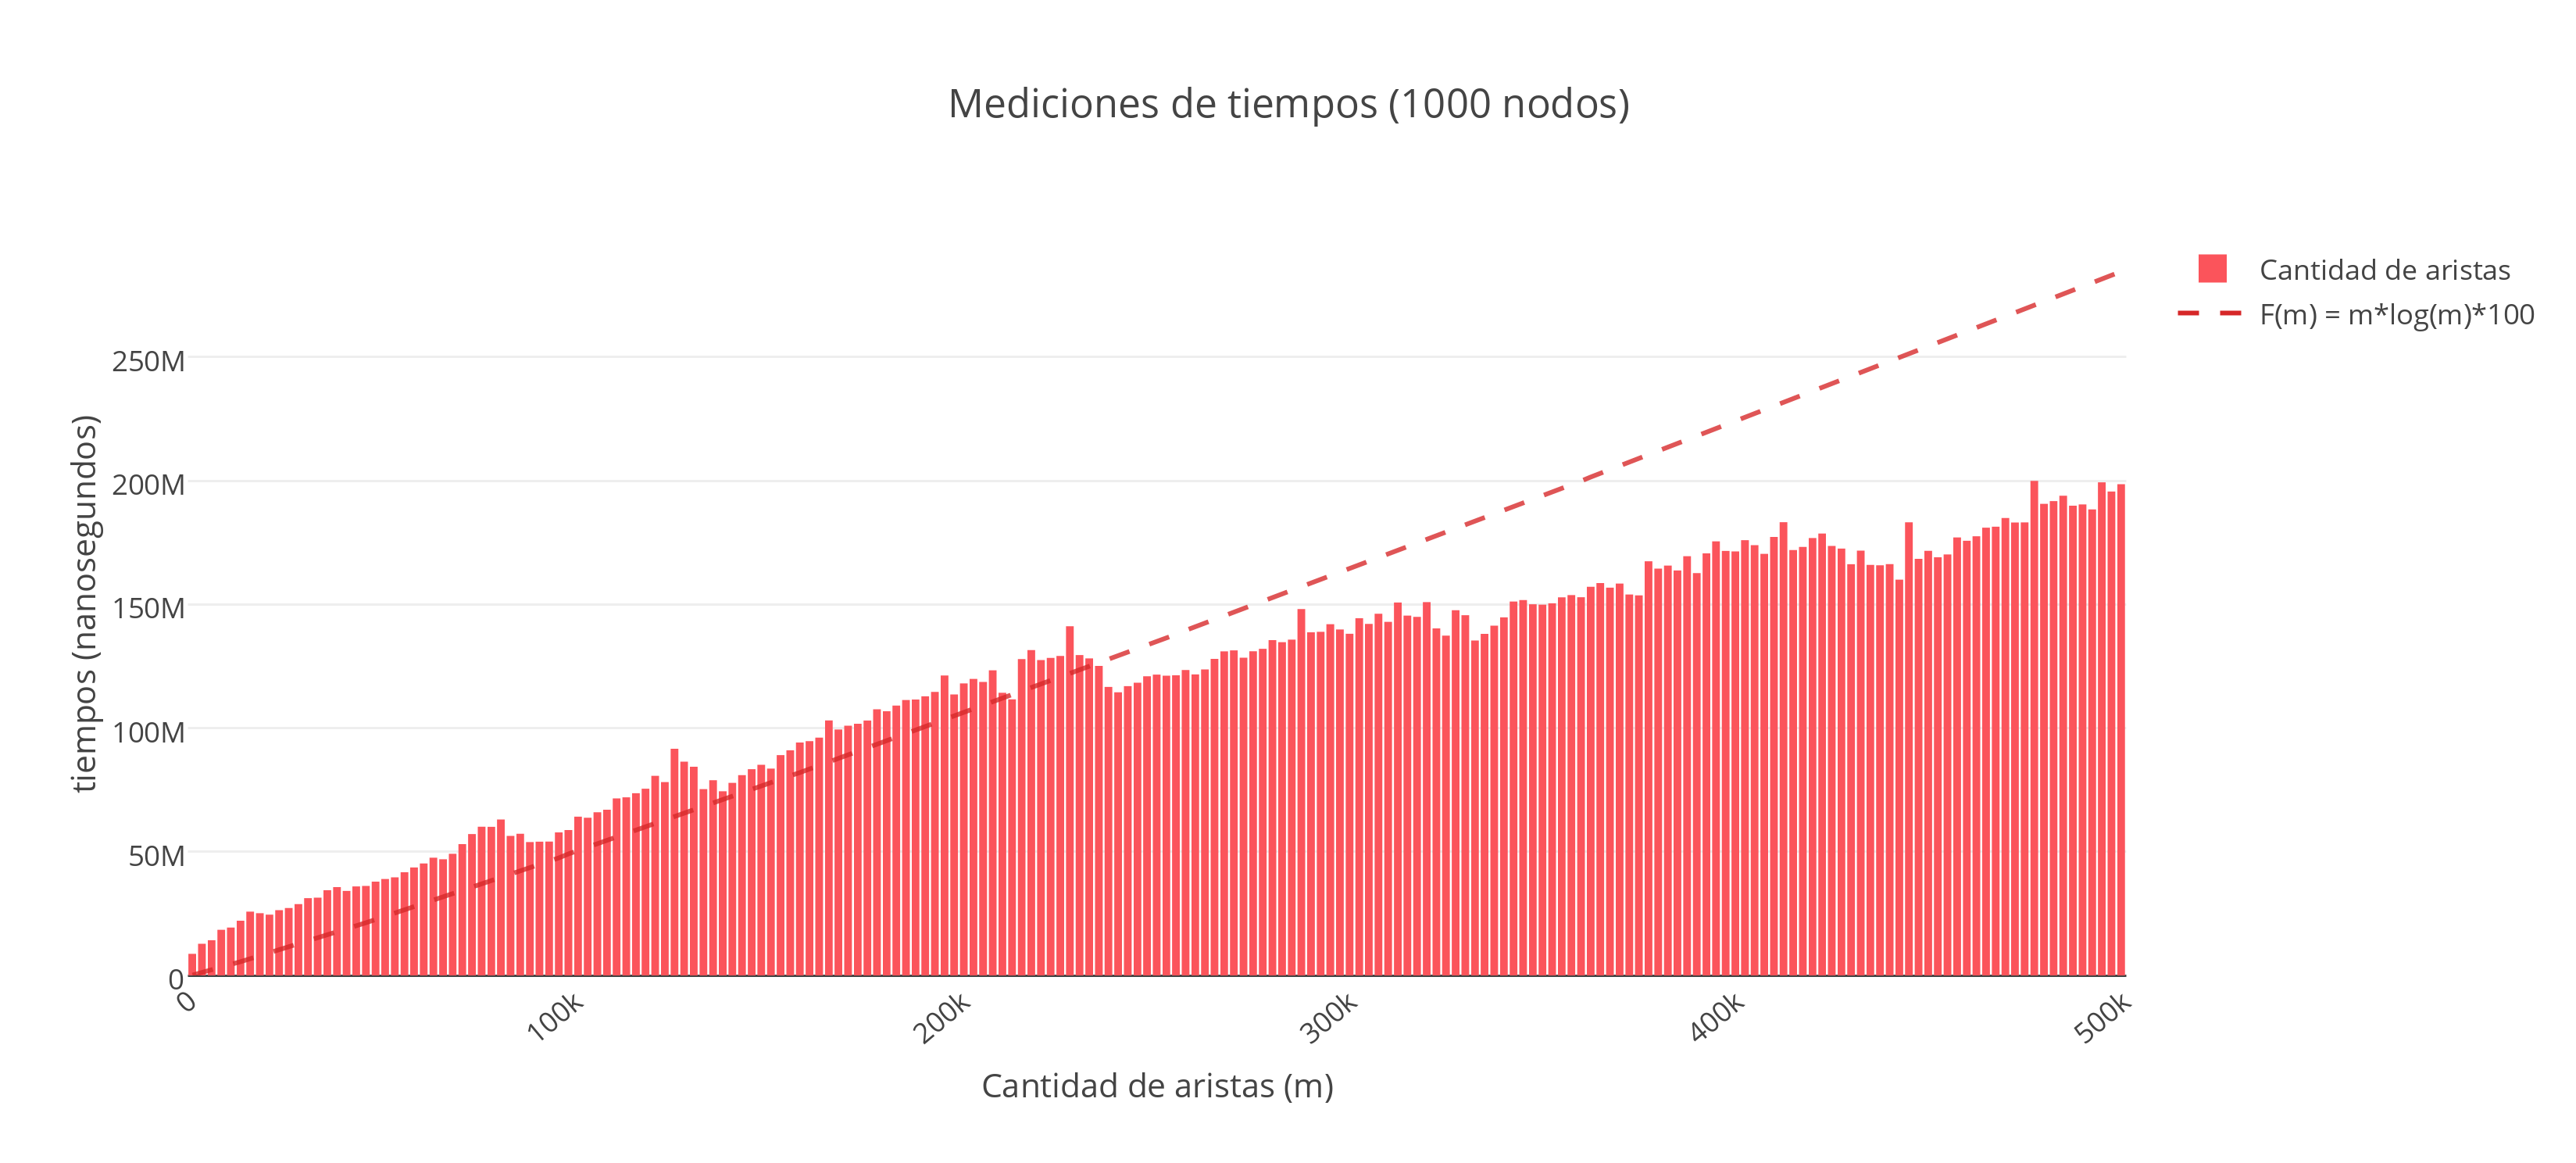
\includegraphics[scale=0.6]{imagenes/ej3/tiempos1000B.png}
% 	\caption{Medición de tiempo promedio con $n$ fijo en 1000}
% 	%\label{tiemposprom}
%  \end{figure}